\section{Ex2.09 Metodo di Eulero}\label{sec:Eulers_method}

\subsection{Testo esercizio}
Spesso si usa il metodo di \textbf{Eulero} per determinare il moto di un oggetto dato 
come l'accelerazione dipende dalla velocità e dalla posizione di un oggetto. 
$$\alpha(x,v) = \mathit{-kx-Cv}$$
Se conosciamo la posizione $\mathit{x}$ e la velocità $\mathit{v}$ in un tempo 
$\mathit{t(0)=0;\;\; x(0)=0\;\; e \;\;v(0)=1}$, possiamo usare il metodo di 
\textbf{Eulero} per trovare la posizione e la velocità dopo un piccolo $\Delta t:$

\begin{displaymath}
\begin{split}
&\mathit{v_1 = v(t_0 + \Delta t) = v(t_0) + \alpha(v(t_0),x(t_0))\Delta t} \\
&\mathrm{x_1 = v(t_0 + \Delta t) = x(t_0) + v(t_0)\Delta t} \\
&\mathsf{v_2 = v(t_1 + \Delta t) = v(t_1) + \alpha(v(t_1),x(t_1))\Delta t} \\
&\mathnormal{x_2 = v(t_1 + \Delta t) = x(t_1) + v(t_1)\Delta t} \\
\end{split}
\end{displaymath}
e cosi via.

\begin{itemize}
    \item[a)] Scrivere una funzione $\mathit{acceleration(x,v,k,C)}$ che restituisce 
    il valore di $\alpha(x,v) = -kx-Cv$.
    
    \item[b)] Scrivi uno script che calcoli i primi $100$ valori di $x(t_i)$ e $v(t_i)$ 
    quando $k=10$, $C=5$ e $\Delta t=0.01$. Traccia $x(t)$, $v(t)$ e $\alpha(t)$ in 
    funzione del tempo.
    
    \item[c)] Modifica la funzione per trovare $x(1)$ e $v(I)$ con    
    $\alpha(x,v)=k\sin(x)-Cv$.    
\end{itemize}

\subsection{Svolgimento}
L'esercizio è stato semplice. Il problema dell'esercizio, ovviamente era la corretta 
scrittura delle formule. Dopo un po' di ragionamento sono arrivata a scriverle 
correttamente. Per il \textit{punto C}, osservata bene la formula ho notato che 
differisce dala precedente solo per $-\sin(x)$ al posto di $x$, per cui ho semplicemente 
richiamato la prima con il $-\sin(x)$ al posto di $x$.

\subsection{Risultati}
\subsubsection{Grafico}
\begin{figure}[h]
    \centering
    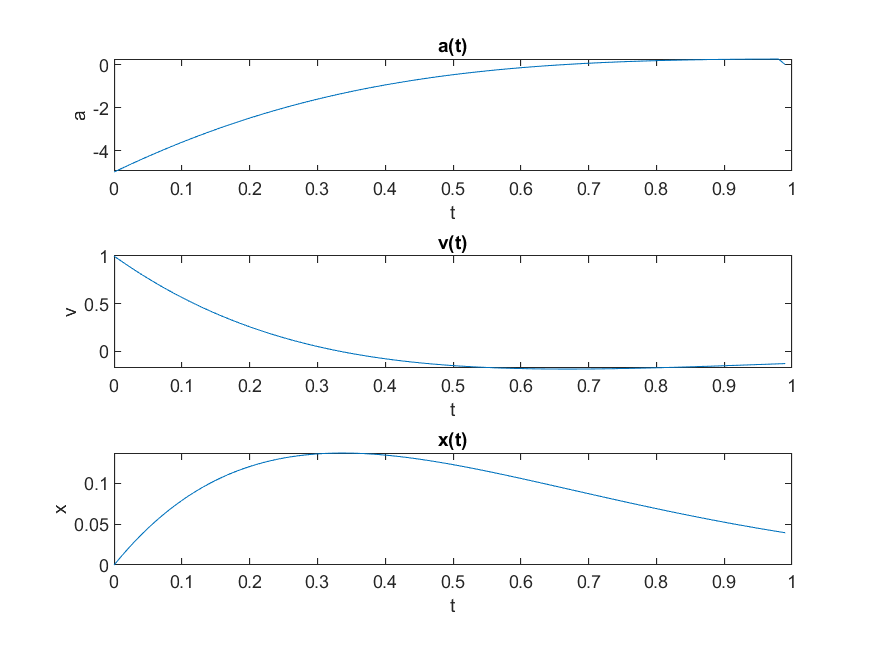
\includegraphics[width=0.7\linewidth]{cap/Elementary/img/script209}
    \GraphCap{$1/x^n$}
    \label{fig:script209}
\end{figure}
\pagebreak
\subsection{Codice esercizio}
\lstinputlisting[caption = {\nameref{fnc:acceleration}},
linerange={1-3}]
{cap/Elementary/src/function/acceleration.m}

\lstinputlisting[title = {script209},
linerange={3-35}]
{cap/Elementary/src/script/script209.m}

\lstinputlisting[title = {\nameref{fnc:acceleration2}},
linerange={1-3}]
{cap/Elementary/src/function/acceleration2.m}

\subsection{CHANGELOG Ex2.09}
\begin{changelog}[author=Cristina, simple, title={Modifiche alla funzione},%
    label=chgf:Eulers_method, sectioncmd=\subsubsection*]
    
    \shortversion{v=3.0.1, date=2020-09-13,%
        changes={Cambiati l'ordine degli argomenti e aggiornata la 
            validazione degli stessi}}      
    
    \shortversion{v=3.0.0, date=2020-09-13,%
        changes={Impostata la variabile \textit{rho} come argomento di 
            input}}
    
    \shortversion{v=2.0.0, date=2020-09-10, changes=Inserita la validazione 
    dell'output}   
    \shortversion{v=1.0.0, date=2020-09-03, changes=Commenti}
    \shortversion{v=0.1.0, date=2020-09-03, changes=Initial beta}
\end{changelog}

\begin{changelog}[author=Cristina, simple, title={Modifiche allo script},% 
    label=chg:script209, sectioncmd=\subsubsection*]
    
    \shortversion{v=1.0.0, date=2020-09-03, changes=Commenti}
    \shortversion{v=0.1.0, date=2020-09-03, changes=Initial beta}
\end{changelog}